%%
%% This is file `main.tex' based on `sample-sigconf.tex' (q.v. for spurce of that,
%%
%% IMPORTANT NOTICE:
%% 
%% For the copyright see the original source file `sample-sigconf.tex'
%% in the `Sample' folder.
%%
%% For distribution of the original source see the terms
%% for copying and modification in the file samples.dtx.
%% 
%% This generated file may be distributed as long as the
%% original source files, as listed above, are part of the
%% same distribution. (The sources need not necessarily be
%% in the same archive or directory.)
%%
%% Commands for TeXCount
%TC:macro \cite [option:text,text]
%TC:macro \citep [option:text,text]
%TC:macro \citet [option:text,text]
%TC:envir table 0 1
%TC:envir table* 0 1
%TC:envir tabular [ignore] word
%TC:envir displaymath 0 word
%TC:envir math 0 word
%TC:envir comment 0 0
%%
%%
%% The first command in your LaTeX source must be the \documentclass command.

%% NOTE that a single column version is required for 
%% submission and peer review. This can be done by changing
%% the \doucmentclass[...]{acmart} in this template to 
%%\documentclass[manuscript,review,anonymous]{acmart}
%% This version is used for drafting and final submission
\documentclass[sigconf]{acmart}
\usepackage{float}


%% 
%% To ensure 100% compatibility, please check the white list of
%% approved LaTeX packages to be used with the Master Article Template at
%% https://www.acm.org/publications/taps/whitelist-of-latex-packages 
%% before creating your document. The white list page provides 
%% information on how to submit additional LaTeX packages for 
%% review and adoption.
%% Fonts used in the template cannot be substituted; margin 
%% adjustments are not allowed.

%%
%% \BibTeX command to typeset BibTeX logo in the docs
\AtBeginDocument{%
  \providecommand\BibTeX{{%
    \normalfont B\kern-0.5em{\scshape i\kern-0.25em b}\kern-0.8em\TeX}}}

%% Rights management information.  This information is sent to you
%% when you complete the rights form.  These commands have SAMPLE
%% values in them; it is your responsibility as an author to replace
%% the commands and values with those provided to you when you
%% complete the rights form.
\setcopyright{acmlicensed}
\copyrightyear{2024}
\acmYear{2024}

%% These commands are for a PROCEEDINGS abstract or paper.
%
%  Uncomment \acmBooktitle if th title of the proceedings is different
%  from ``Proceedings of ...''!
%
%\acmBooktitle{Woodstock '18: ACM Symposium on Neural Gaze Detection,
%  June 03--05, 2018, Woodstock, NY} 
\acmISBN{978-1-4503-XXXX-X/18/06}


%%
%% Submission ID.
%% Use this when submitting an article to a sponsored event. You'll
%% receive a unique submission ID from the organizers
%% of the event, and this ID should be used as the parameter to this command.
%%\acmSubmissionID{123-A56-BU3}

%%
%% For managing citations, it is recommended to use bibliography
%% files in BibTeX format.
%%
%% You can then either use BibTeX with the ACM-Reference-Format style,
%% or BibLaTeX with the acmnumeric or acmauthoryear sytles, that include
%% support for advanced citation of software artefact from the
%% biblatex-software package, also separately available on CTAN.
%%
%% Look at the sample-*-biblatex.tex files for templates showcasing
%% the biblatex styles.
%%

%%
%% The majority of ACM publications use numbered citations and
%% references.  The command \citestyle{authoryear} switches to the
%% "author year" style.
%%
%% If you are preparing content for an event
%% sponsored by ACM SIGGRAPH, you must use the "author year" style of
%% citations and references.
%% Uncommenting
%% the next command will enable that style.
%%\citestyle{acmauthoryear}

%%
%% end of the preamble, start of the body of the document source.

%% % Location of your graphics files for figures, here a sub-folder to the main project folder
\graphicspath{{./images/}} 


\begin{document}

%%
%% The "title" command has an optional parameter,
%% allowing the author to define a "short title" to be used in page headers.
\title{Competitive Esports Network: A Relational Approach to
Tournament Management \\ Phase IV}

%%
%% The "author" command and its associated commands are used to define
%% the authors and their affiliations.
%% Of note is the shared affiliation of the first two authors, and the
%% "authornote" and "authornotemark" commands
%% used to denote shared contribution to the research.
\author{Wyatt Fischer}
\email{fisc7842@vandals.uidaho.edu}
\affiliation{
    \institution{University of Idaho}
    \city{Moscow}
    \state{Idaho}
    \country{USA}
}

\author{Nastia Kossiak}
\email{koss0519@vandals.uidaho.edu}
\affiliation{
    \institution{University of Idaho}
    \city{Moscow}
    \state{Idaho}
    \country{USA}
}
\author{Brandon Lunney}
\email{lunn2076@vandals.uidaho.edu}
\affiliation{
    \institution{University of Idaho}
    \city{Moscow}
    \state{Idaho}
    \conutry{USA}
}

%%
%% By default, the full list of authors will be used in the page
%% headers. Often, this list is too long, and will overlap
%% other information printed in the page headers. This command allows
%% the author to define a more concise list
%% of authors' names for this purpose.
\renewcommand{\shortauthors}{Fischer, Kossiak, and Lunney}

%%
%% The abstract is a short summary of the work to be presented in the
%% article.
\begin{abstract}
The final report for the E-Sports Competitive Network is presented. A tool which is designed to showcase player, team, and tournament's dynamic relationships through a graphical interface and underlying relational database. The report includes a finalized prototype description detailing all the features included within the finished product. The finalized entity relation model with discussion on changes from the initial design. A finalized tech stack from the database to the front end. Implementation details for each of the custom web scrappers that populate the database. Discussion on each of the three core analytical queries provided by the tool. Including showcases of all web pages of the project. Lastly, a reflection on the initial timeline with a phase by phase break down on the project's development. 
\end{abstract}

%%
%% The code below is generated by the tool at: http://dl.acm.org/ccs.cfm
%% Please copy and paste the code instead of the example below.
%%
\begin{CCSXML}
<ccs2012>
 <concept>
  <concept_id>00000000.0000000.0000000</concept_id>
  <concept_desc>Information Systems</concept_desc>
  <concept_significance>500</concept_significance>
 </concept>
 <concept>
  <concept_id>00000000.00000000.00000000</concept_id>
  <concept_desc>Applied Computing</concept_desc>
  <concept_significance>300</concept_significance>
 </concept>
</ccs2012>
\end{CCSXML}

\ccsdesc[500]{Relational Databases}
\ccsdesc[300]{Computer Games}

%%
%% Keywords. The author(s) should pick words that accurately describe
%% the work being presented. Separate the keywords with commas.
\keywords{Esports, Relational Databases, MySQL, Cytoscape, Network Visualization, Python}

%%
%% This command processes the author and affiliation and title
%% information and builds the first part of the formatted document.
\maketitle

\section{Introduction}
E-Sports is one of the fastest growing media in recent years. The biggest e-sports events can even receive upwards of 5.5 million views. With a wide range of games, including titles such as \textit{League of Legends}, \textit{Counter-Strike}, and \textit{Dota 2}, the industry has developed a vast ecosystem of professional teams and large-scale tournaments. However, unlike it's real life counterpart e-sports does not have near the amount of statistical analysis tools as regular sports. These tools allow coaches, fans, and researchers to better understand performance trends, strategic strengths, and the relationships between teams across seasons. This was the motivation behind the \textit{E-Sports Competitive Network}. For this project we will be implementing a relational database to facilitate statistical analysis of e-sports players and teams across several seasons and games. We will then utilizing that database to visually communicate the information in a graph format.\\
The requirements of this project are we facilitate multiple types of nodes, in this instance this is players, teams, and the tournaments themselves. This project will also allow for several edges types, such that teammates, played in, and played for. We also allow for multi-graph support, specifically the ability for a node to belong to several graphs and by extension edges to multiple graphs as well. There will also feature a minimum set of queries available, such as an h-index filter or for our purposes a win rate filter for the teams and players. As well as a Co-Author network which for this system will be a teammate network.  Lastly, there will be a Q1 journal influence network. However, for our purposes this will be a Q1 tournament influence network, where the Q1-Q4 will be determined based on which quartile the prize pool falls into. Then we will find all teams and by extension the players that participated in that tournament.
\section{Final Prototype Description}
This report covers the final prototype of the Competitive Esports Network. The E-Sports Competitive Network final prototype is designed to address the lack of advanced statistical analysis tools in competitive gaming. This prototype introduces a relational database system that models graph connections between players, teams, and tournaments across multiple games. This prototypes implements three key queries which can be applied onto the project's database. First, we have a teammate network query. This query was based off the \textit{Co-Author Network} query seen in several journal analytical tools, allowing for a visualization of player interactions and relationships. The second query this project includes is an h-index filter. Based on the analytical query with the same name this query allows for both tournament participation and tournament wins filters. Allowing for an analytical analysis of team performance. The final query is a Q1 tournament influence network, which is based on a Q1 journal influence network. Which allows for tournaments to be filtered into Q1 status and then get all teams that participated in that tournament. Allowing for a measurement of a tournament's impact. Aside from the three primary queries the final prototype features several web pages to display the contents of the queries as well as allow for input into the database manually. We have also built several web scrappers to populate the database with data.
\section{Final Entity Relation Model}
The final entity relation model looks vastly different than the initial model, as seen in figure 1. Initially we planned on having each different type of data, player, team, and tournament, represent its own table. In addition with the respective relationships between the data points. This worked fine for the basic prototype which allowed for basic create, read, update, and delete operations within the database. However, as we implemented more of the graph front end this schema did not hold up. This lead to complex queries to get the appropriate information for Cytoscape and did not allow for multi-graph support. Therefor we ended up with the final model depicted in Figure 2.
\begin{figure}[H]
    \centering
    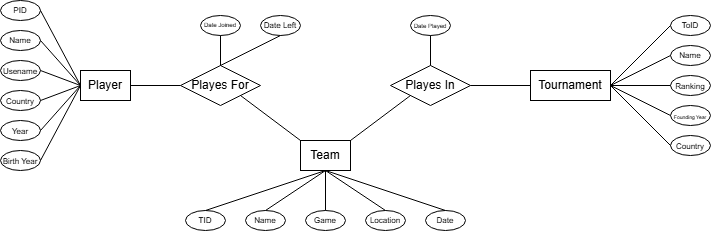
\includegraphics[width=1\linewidth]{images/ERDiagram.png}
    \caption{Initial Entity Relation Diagram}
    \label{fig:placeholder}
\end{figure}

\begin{figure}[H]
    \centering
    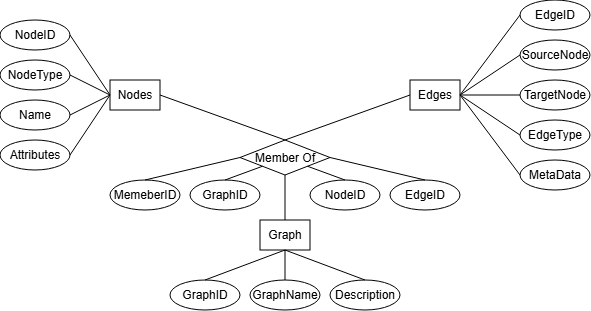
\includegraphics[width=1\linewidth]{images/UpdatedERDiagram.png}
    \caption{Finalized Entity Relation Model}
    \label{fig:placeholder}
\end{figure}

The benefits of this model is rather than having three different types of entities for each team, player, and tournament we simply have a Node entity. Each Node has a NodeID which acts as the primary key. Then the team, player, or tournament attribute is stored withing the NodeType value. Since each team, player, and tournament has different amount of attributes stored with it the Attributes column is a JSON file allowing for flexible metadata on the node. \\
Similarly, rather than having two different tables for the played-for and played-in relationship we consolidated it to one Edge entity. Each edge has a an EdgeID acting as the primary key. As well as two node id's, SourceNodeID and TargetNodeID, which describe the nodes the edge connects as well as are foreign keys to the node table. For the same reasons as the node entity we gave the edge entity and EdgeType value which holds the played-in or played-for relationship. Lastly, since each relasonship holds a different number of descriptors edges have a MetaData value which acts identically to the Attributes column of nodes.\\
To facilitate the multi-graph support we've added a new entity to represent the graphs themselves. Each graph has a GraphID which is the primary key of the table. Each graph also has a name that can be displayed. In addition, each graph has a description to further add details to the graph.
We've also added a new relationship between the entities, Member of, this represents the relationship between a graph and a node or edge. Each membership has it's own MemeberID which acts as the primary key. A nodeID or edgeID which determines which entity belongs to the graph. The graphID to determine which graph the entity belongs to. This schema allows for easy graph integration and multi-graph support, in addition for further expansion if we decide to add more types of nodes or edges.
\section{Tech Stack}

\subsection{Database}
Initially the database we decided on was \textbf{MySQL}, which is based around the client-server model. To simplify development and improve collaboration we've transitioned to \textbf{SQLite}, a lightweight relational database that follows a serverless architecture. This design makes it extremely easy to set up and allows team members to share the database simply by distributing the file.
\subsection{Back-End}
For the back end we've utilized \textbf{Python} for it's expansive libraries and data analysis tools. We leveraged Python’s frameworks and libraries to handle core logic and data interaction with the SQLite database. Discussed later, we utilized Flask for webpage routing and Playwright to populate the database.
\subsection{Front-End}
The front end utilizes HTML and CSS for the webpage templates as well as the presentation. To present the graph presentation of the network we utilize Cytoscape which is an open-source network visualizer. Which allows us to render complex relationships in an intuitive way. Through its JavaScript integration we are able to embed interactive graphs directly into the webpage.

\section{Implementation}
\subsection{Populating the Database}
To populate the initial database we've developed a web scrapper that utilizes Playwright to load web pages and scrape the information from the html tags then inserts them into the database. The scraper checks for duplicate nodes, in that case the node's attributes are updated. In addition, the scrapper creates the respective edges as well. Below is a list of webpages where we scrape the information.

\begin{enumerate}
    \item https://prosettings.net/players/
    \item https://en.wikipedia.org/wiki/
    \item https://liquipedia.net/valorant/S-Tier\_Tournaments
    \item https://liquipedia.net/fortnite/S-Tier\_Tournaments
    \item https://liquipedia.net/dota2/Tier\_1\_Tournaments
    \item https://liquipedia.net/counterstrike/S-Tier\_Tournaments
    \item https://liquipedia.net/rainbowsix/S-Tier\_Tournaments
    \item https://liquipedia.net/pubg/S-Tier\_Tournaments
    \item https://liquipedia.net/apexlegends/S-Tier\_Tournaments
    \item https://liquipedia.net/rocketleague/S-Tier\_Tournaments
    \item https://liquipedia.net/leagueoflegends/S-Tier\_Tournaments
\end{enumerate}
\subsubsection{Player Web Scrapper}
The web scrapper designed to collect Player information gathers its information from link (1), it starts by creating the respective tables if needed, Nodes and Edges. Then, after establishing the database connection, utilizes playwright to start a Mozilla 5.0 instance. Then ignores heavy resources such as images, fonts, and other media. Then utilizing a regex statment pulls finds all locations on the document that match \textit{'a[href*="/players/"]'}. This is then cleaned to remove the player's game information information, leaving a ready to process url. The scrapper also checks if no new players are added as well. Once there are no new players added from scrapping the scrapper moves to inserting the information. Each of the grabbed urls is then loaded individually. The scrapper then pulls the table tags from the page. Then iterates through the table rows and columns collecting the player's real name, birthday, and country or Unknown if the information is null. Lastly, it collects the team the player belongs to or assumes "Free Agent" if the do not belong to a team. Once the information has been collected the following queries are executed. The first query is to check if the information has already been inserted. If it has been inserted the information is updated with the second query. If it is not present in the database the last query is executed to insert the information into the database.
\begin{verbatim}
    SELECT NodeID
    FROM Nodes
    WHERE Name = $username
    AND NodeType = 'Player';

    UPDATE Nodes
    SET Attributes = $player_attributes
    WHERE NodeID = $player_id;

    INSERT INTO Nodes
    (NodeType, Name, Attributes)
    VALUES ('Player', $username, $player_attributes);
\end{verbatim}
Since many players may belong to one team the scrapper also checks to make sure the same team is not inserted several times. It does this with the below queries. The first one checks if the team has already been inserted, in the event it has not been inserted the second query is executed.
\begin{verbatim}
    SELECT NodeID
    FROM Nodes
    WHERE Name = $team_name
    AND NodeType = 'Team'

    INSERT INTO Nodes
    (NodeType, Name, Attributes)
    VALUES ('Team', $team_name, $team_attributes)
\end{verbatim}
Once this has been executed the last thing the scrapper needs to do it insert relevant edge information. This is done by the below queries, the first checks if the edge has already been inserted. If it is not present the second is executed.
\begin{verbatim}
    SELECT EdgeID
    FROM Edges
    WHERE SourceNodeID = $player_id
    AND TargetNodeID = $team_id
    AND EdgeType = 'Plays_For'

    INSERT INTO Edges
    (SourceNodeID, TargetNodeID, EdgeType)
    VALUES ($player_id, team_id, 'Plays_For');
\end{verbatim}
This process is repeated for each of the player urls that get scrapped during the initial url collection. Once this is completed the scrapper has been completed.
\subsubsection{Teams Web Scrapper}
The teams web scrapper is designed to collect as well as fill in missing team information from link (2). The scrapper starts by creating the needed tables if need as well as establishing the database connection. Once that has been completed the below query is executed, which pulls teams that are missing location or founded attributes.
\begin{verbatim}
    SELECT NodeID, Name, Attributes 
    FROM Nodes 
    WHERE NodeType = "Team" 
    AND (Attributes NOT LIKE '%"location"%' 
    OR Attributes NOT LIKE '%"founded"%')
\end{verbatim}
For each of the teams with partial information it pulls what information is present then loads the respective wikipedia page. Since some pages have inconsistent naming schemes the scrapper is designed to check both \textit{/wiki/\$teamname} and \textit{/wiki/\$teamname\_(esports)}. Once the page is loaded the scrapper pulls from the respective table on the page, aiming to gather the location and founder information if present. Once the wikipedia information is collected the below query is executed. If the Wikipedia page was found then the attributes are updated with the found information. If the page could not be found the attributes are updated with the \textit{wiki\_found} value set as false.
\begin{verbatim}
    UPDATE Nodes 
    SET Attributes = $attrs 
    WHERE NodeID = $teamID
\end{verbatim}
Once this is completed for all teams with missing information then the scrapper is finished.
\subsubsection{Tournament Web Scrapper}
Lastly the tournament web scrapper is designed to gather tournament information from links (3) through (11). Similar to the other two the scrapper starts by creating the respective tables if necessary and establishes the database connection. Playwright is then used to initialize the browser instance. Then for each of the games and it's respective url, the browser opens the game's website loading the table present on the page. For each row in the table it gathers only the tournaments that are gold highlighted, collecting the tournament's url, date, prize pool, location, and winner information. The scrapper does not collect tournaments that have not happened yet. Once all the information has been gathered the first query is executed to insert the information. If the tournament is already present the second query is executed. Lastly the winning team is inserted into the database as well.
\begin{verbatim}
    INSERT OR IGNORE INTO Nodes
    (NodeType, Name, Attributes)
    VALUES ('Tournament', $tournament_name, $attr_json)

    UPDATE Nodes
    SET Attributes = $attr_json
    WHERE Name = $tournament_name
    AND NodeType = 'Tournament'
    
    INSERT OR IGNORE INTO Nodes
    (NodeType, Name, Attributes)
    VALUES ("Team", $winner, $game_attributes);
\end{verbatim}
Next the scrapper moves to insert relevant edge information. The below queries are executed, the first query is used to get the appropriate node information for the given tournament from the database. Then the winning team's information is gathered with the second query. Then the scrapper adds both a \textit{Won By} and \textit{Played In} edge into the edges table connecting the tournament and winning team. This is accomplished by the third and fourth queries. The same process is repeated for the runner up team, but does not add the \textit{Won By} edge. This is completed by the fifth and sixth queries. Once this is executed for every tournament for each of the games listed in the links table the web scrapper is complete.
\begin{verbatim}
    SELECT NodeID
    FROM Nodes
    WHERE Name = $tournament_name
    AND NodeType = "Tournament"

    SELECT NodeID
    FROM Nodes
    WHERE Name = $winner
    AND NodeType = "Team"

    INSERT OR IGNORE INTO Edges
    (SourceNodeID, TargetNodeID, EdgeType)
    VALUES ($tournament_ID, $winner_ID, 'Won_By')

    INSERT OR IGNORE INTO Edges
    (SourceNodeID, TargetNodeID, EdgeType)
    VALUES ($tournament_ID, $winner_ID, 'Played_In')
    
    SELECT NodeID
    FROM Nodes
    WHERE Name = $runner_up
    AND NodeType = "Team"

    INSERT OR IGNORE INTO Edges
    (SourceNodeID, TargetNodeID, EdgeType)
    VALUES ($tournament_ID, $runner_up_ID, 'Played_In')
\end{verbatim}

In addition to the web scraper, the project also includes several dedicated webpages that allow users to insert data directly into the database. These pages utilize forms to fill in a SQL statement that is then executed by the database manager. Figures 3 showcases the database insertion webpages.

\begin{figure}[H]
    \centering
    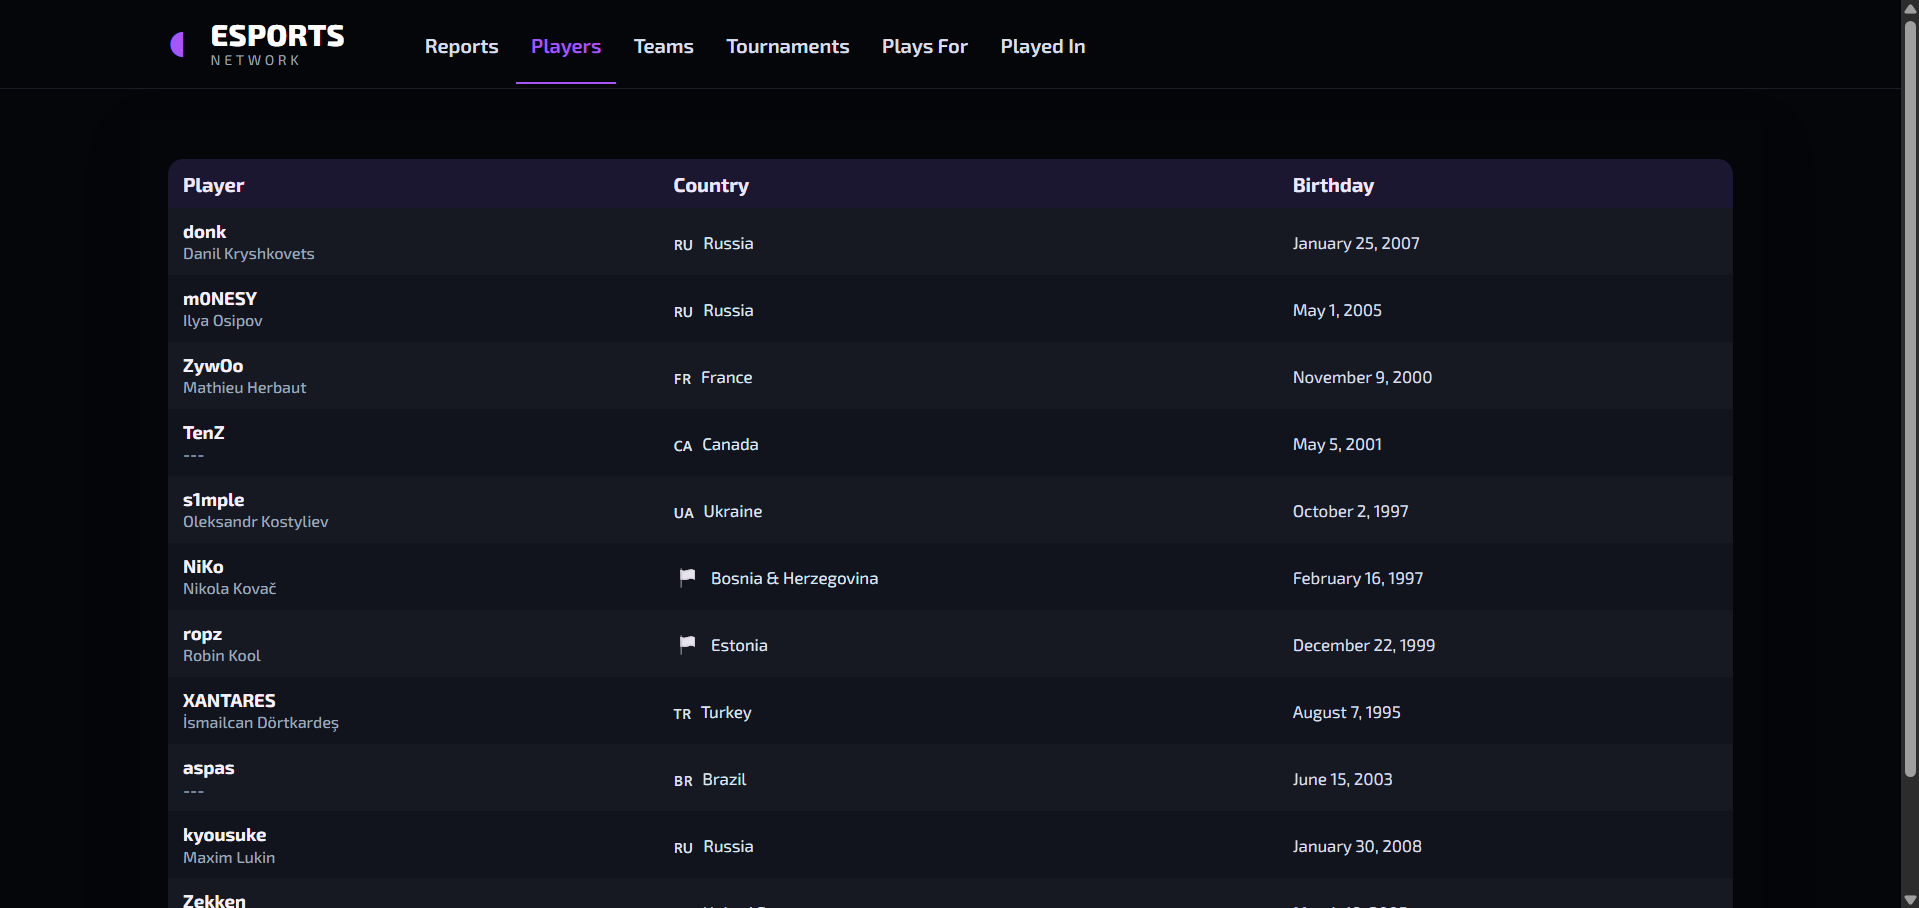
\includegraphics[width=1\linewidth]{images/ESports-Players.png}
    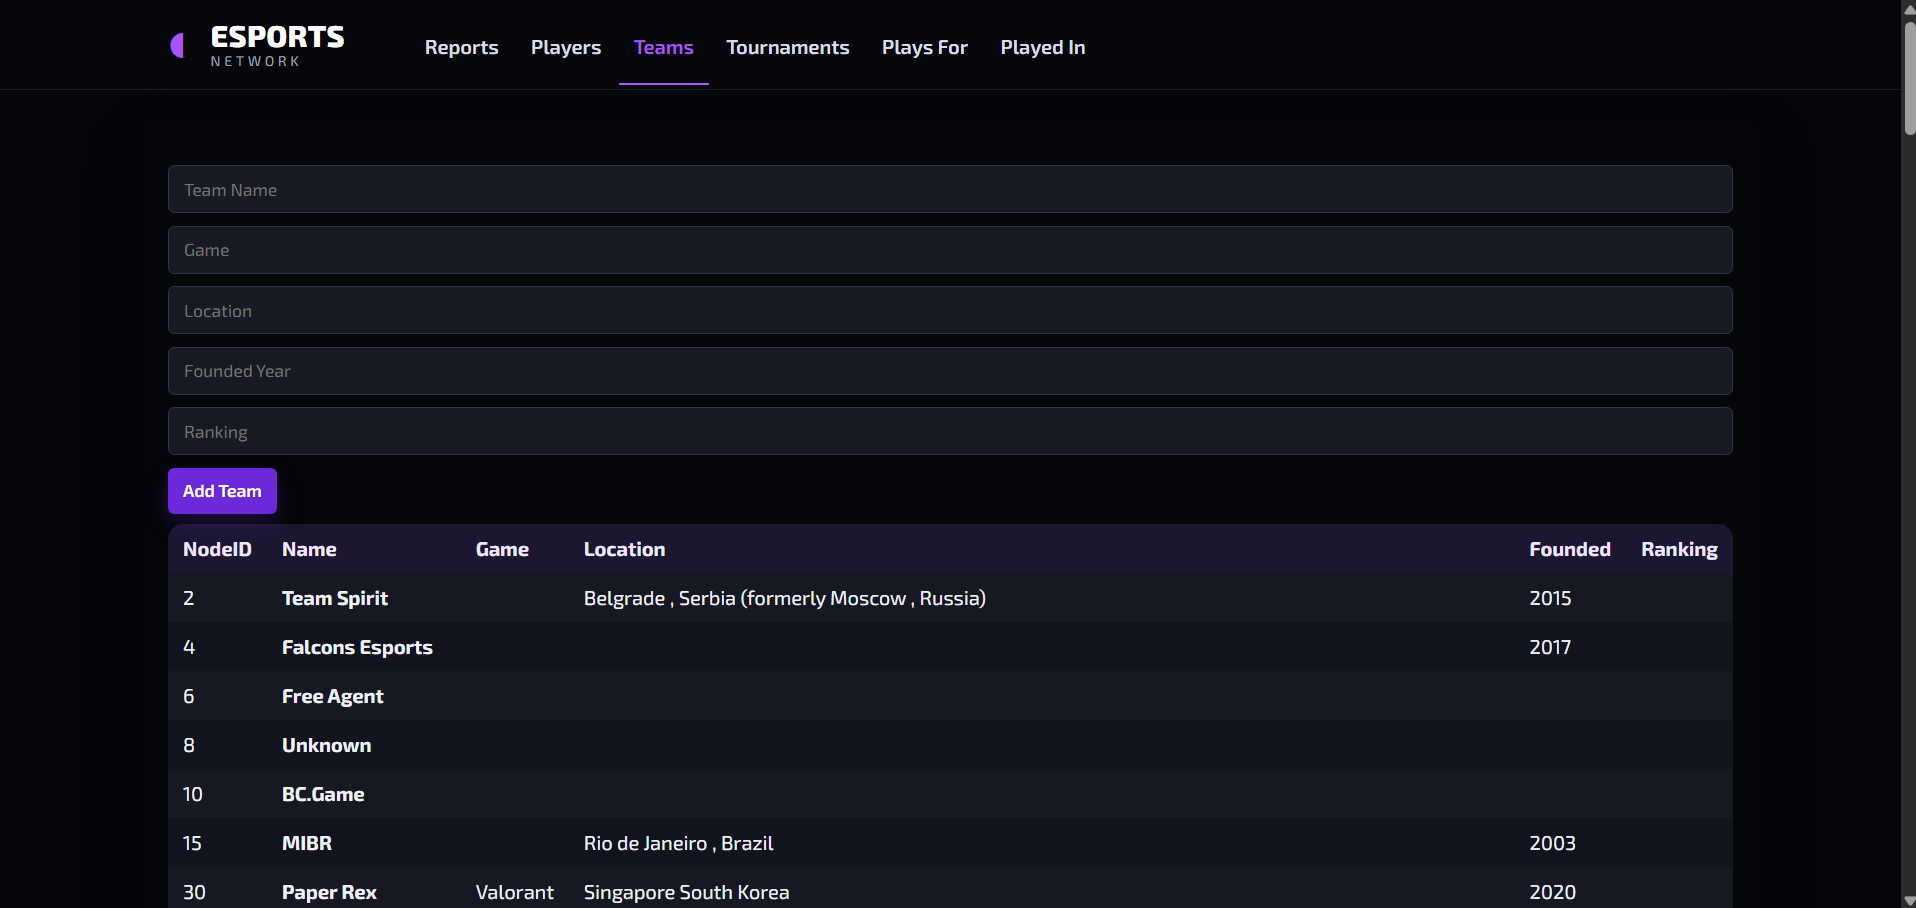
\includegraphics[width=1\linewidth]{images/ESports-Teams.png}
    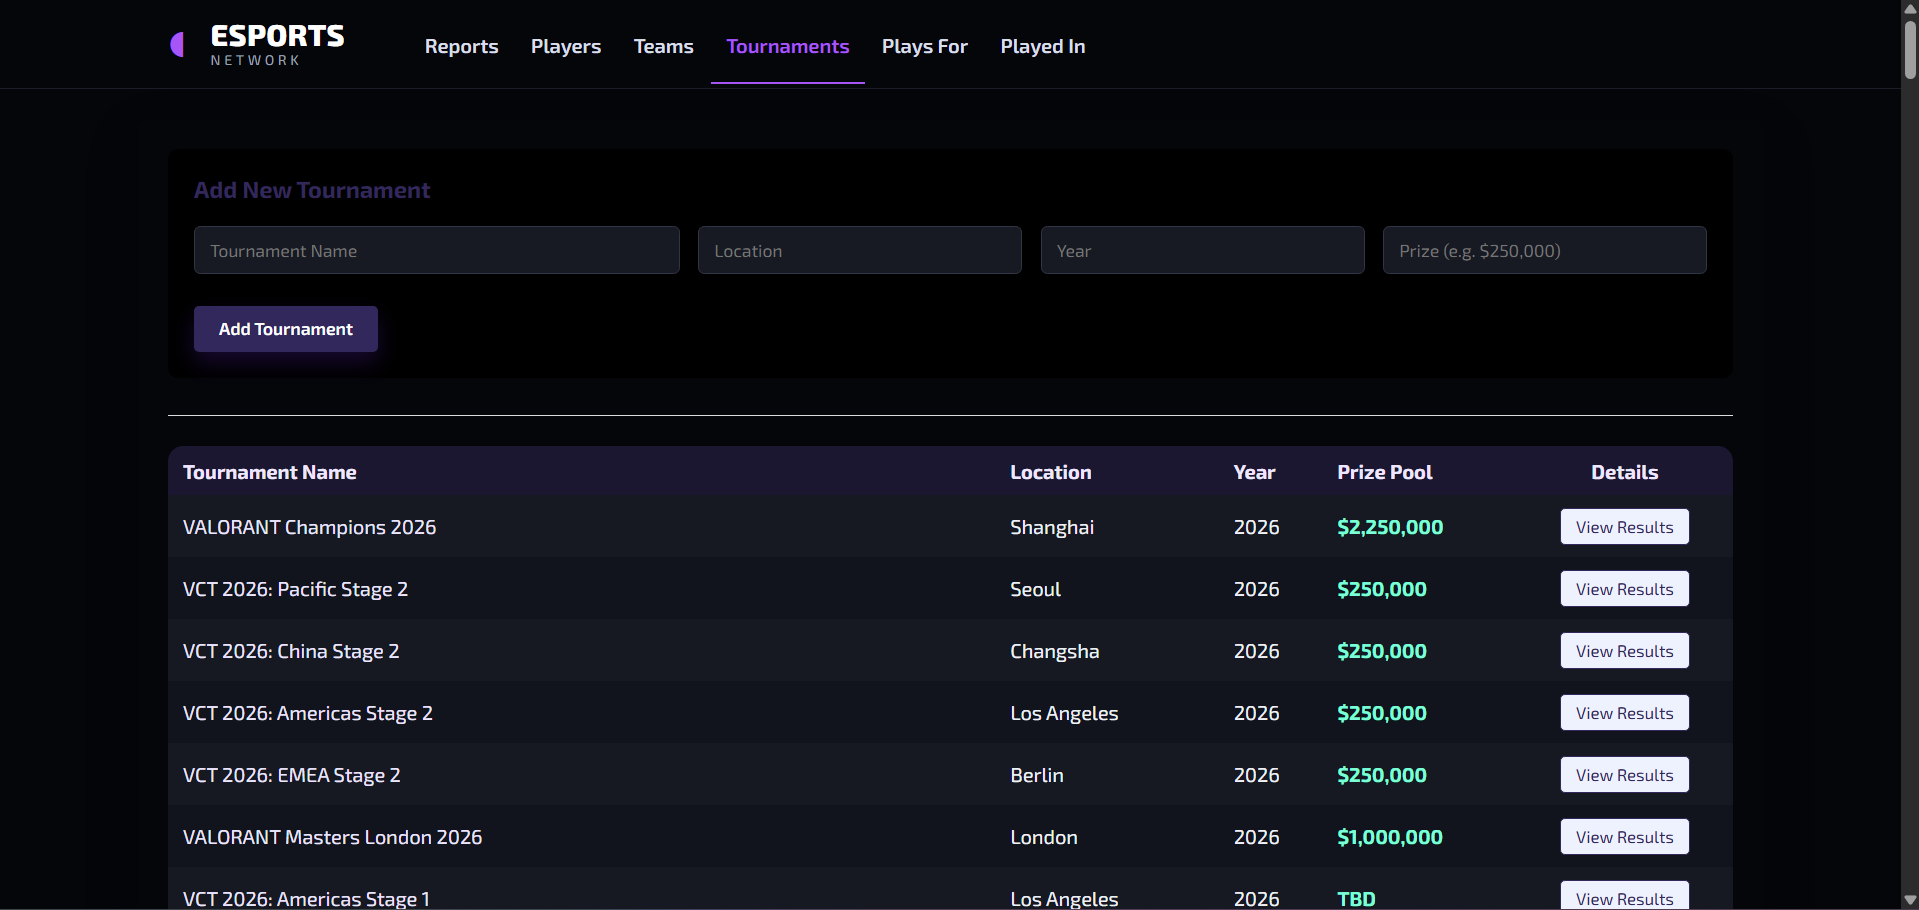
\includegraphics[width=1\linewidth]{images/ESports-Tournaments.png}
    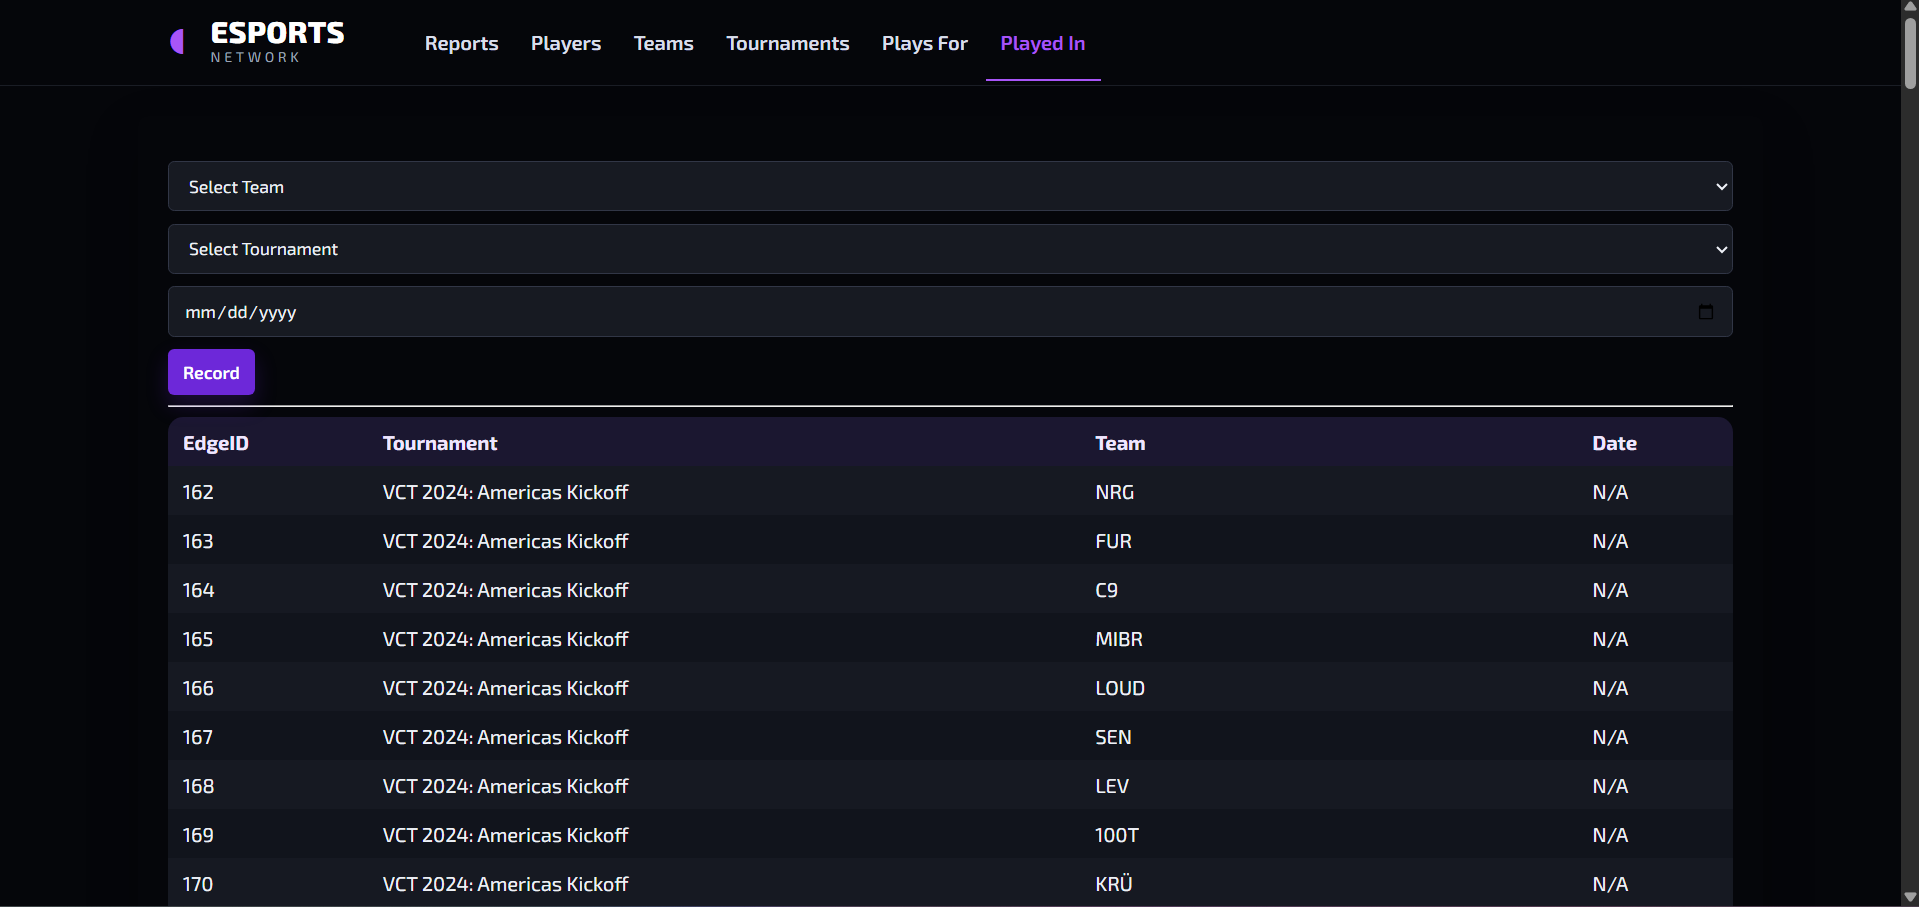
\includegraphics[width=1\linewidth]{images/ESports-PlayedIn.png}
    \label{fig:placeholder}
\end{figure}
\begin{figure}[H]
    \centering
    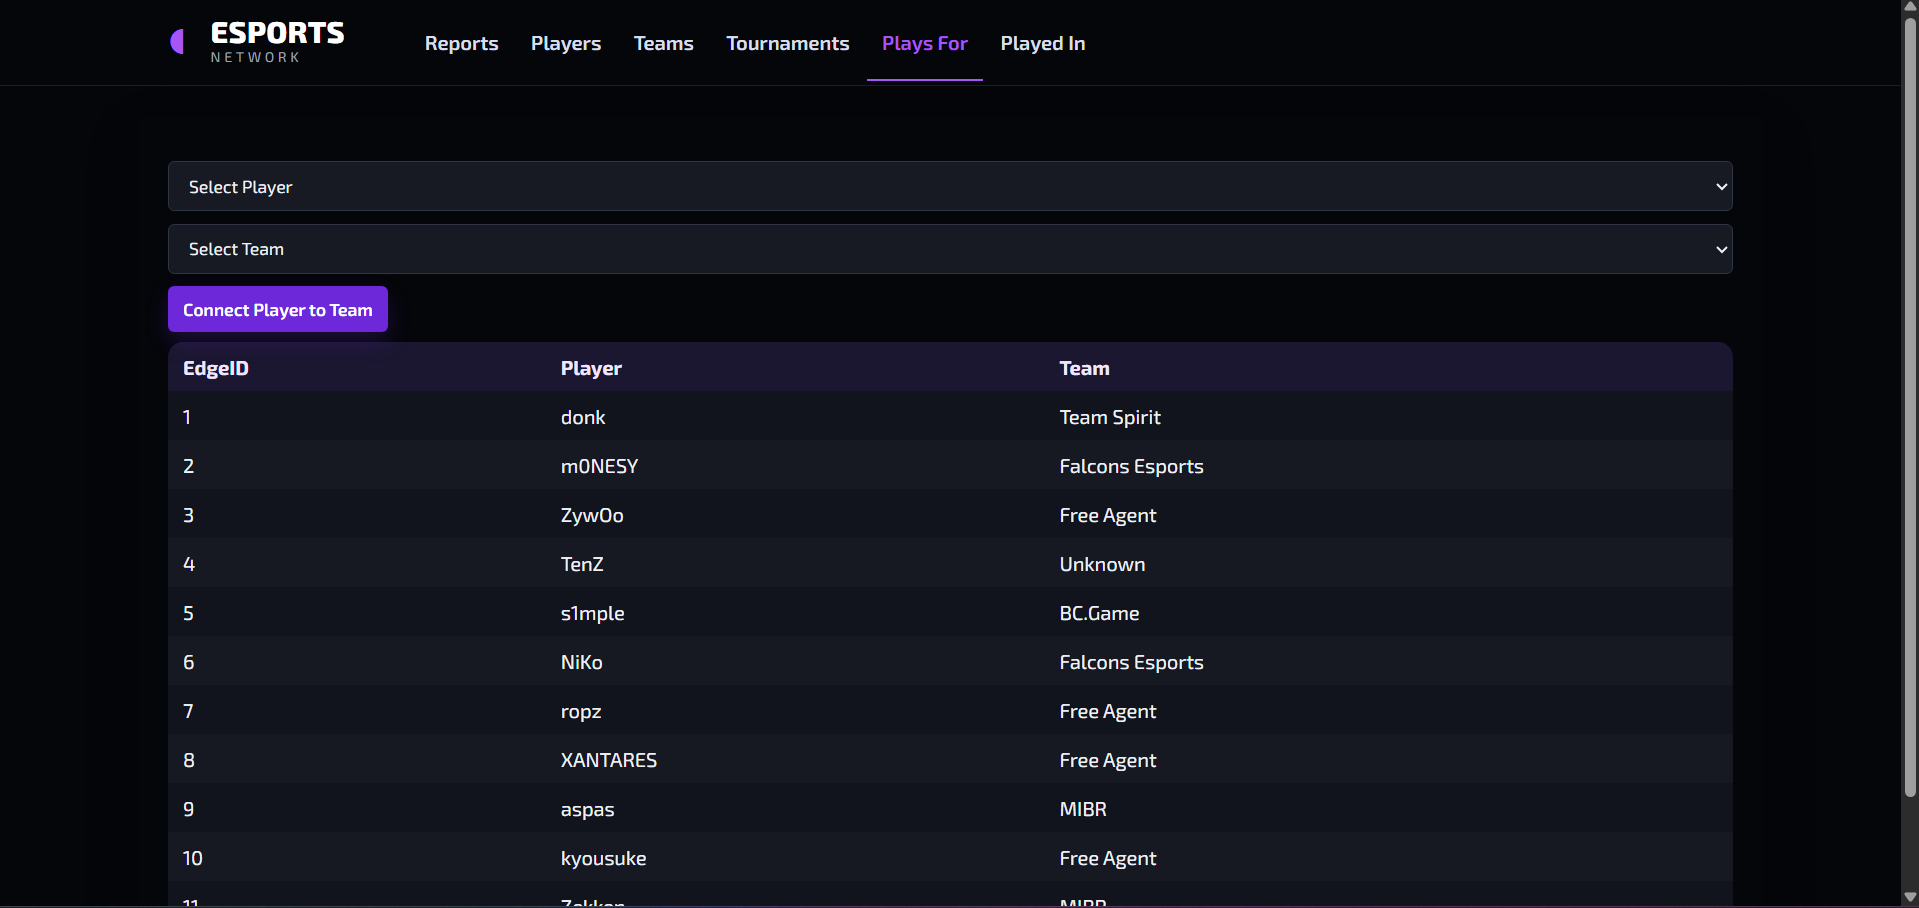
\includegraphics[width=1\linewidth]{images/ESports-PlaysFor.png}
    \caption{Database Insertion Webpages}
    \label{fig:placeholder}
\end{figure}

\subsection{Reports Page}
As mentioned previously the project utilizes Flask to handle webpage routing. Each webpage calls from the database and then fills in the template html page with the returned information from the database. The front page get the entire database then utilizes Cytoscape's java script integration to present the information. Figure 4 showcases the front webpage.
\begin{figure}[H]
    \centering
    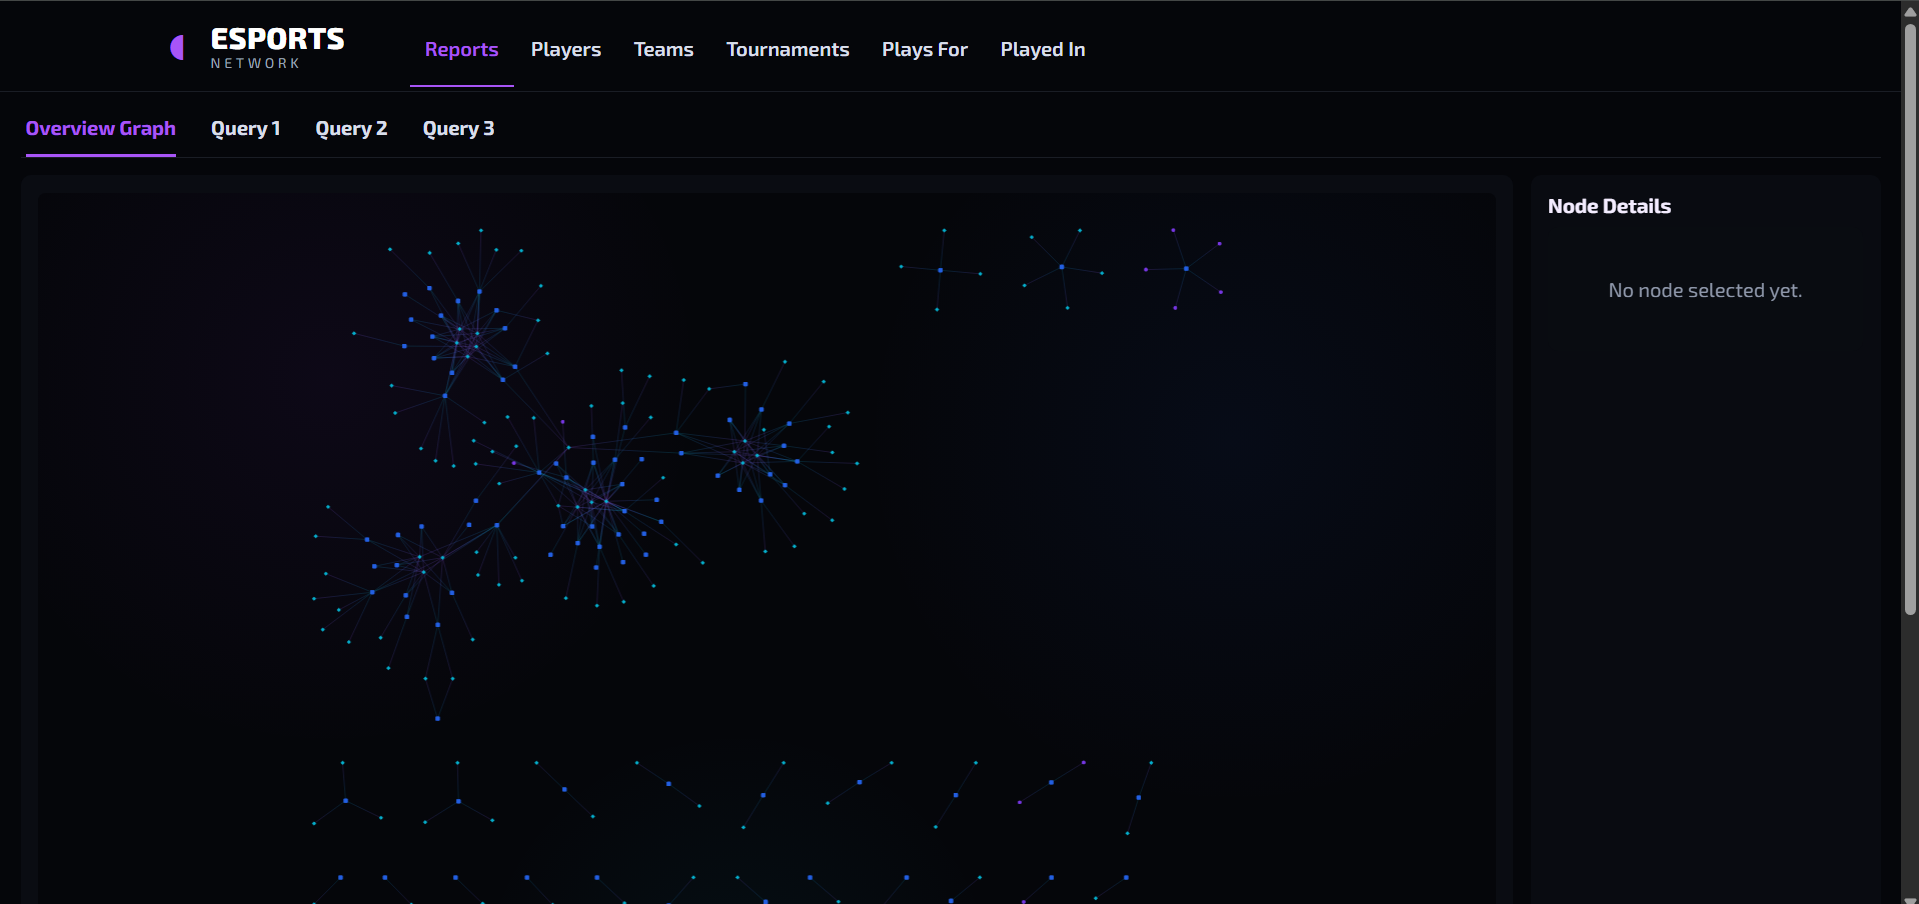
\includegraphics[width=1\linewidth]{images/ESports-Reports.png}
    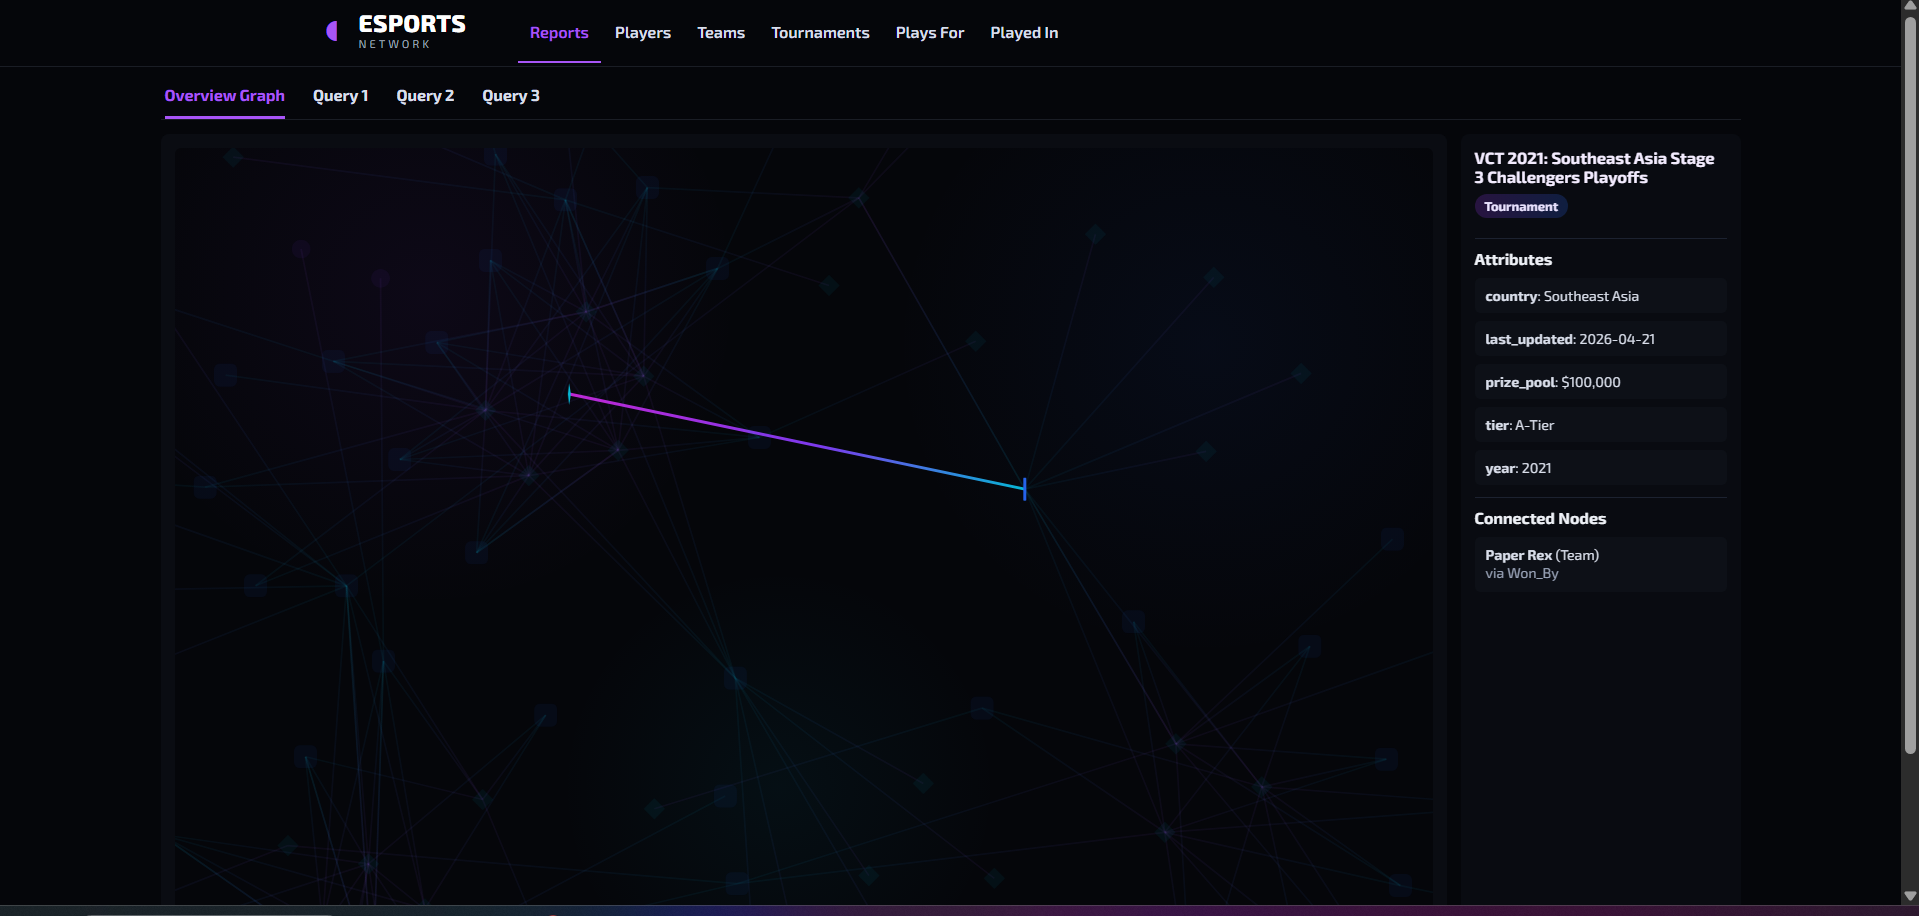
\includegraphics[width=1\linewidth]{images/ESports-ReportsExample.png}
    \caption{Reports Web Page}
    \label{fig:placeholder}
\end{figure}

\subsection{Query 1}
For this project the first analytical query we implemented was a \textit{Teammate Network}. This is based on a similar concept of a \textit{Co-Author Network} used by research paper databases. This query is used to visualize the player's relationships and interactions. The below queries are executed when completing the query. Given a specific player we find all node that are connected the same matching team with the \textit{Plays For} edge. Figure 5 showcases the query web pages themselves.

\begin{verbatim}
SELECT DISTINCT n.NodeID, n.Name, n.NodeType, n.Attributes
    FROM Nodes n
    JOIN GraphMemberships gm ON gm.NodeID = n.NodeID
    WHERE gm.GraphID = 1
    AND n.NodeType IN ("Player", "Team")
    ORDER BY n.NodeType, n.Name
SELECT DISTINCT e.EdgeID, e.SourceNodeID, e.TargetNodeID, 
e.EdgeType, e.Metadata
    FROM Edges e
    JOIN GraphMemberships gm ON gm.EdgeID = e.EdgeID
    WHERE gm.GraphID = 1
    AND e.EdgeType = "Plays_For"
\end{verbatim}

\begin{figure}[H]
    \centering
    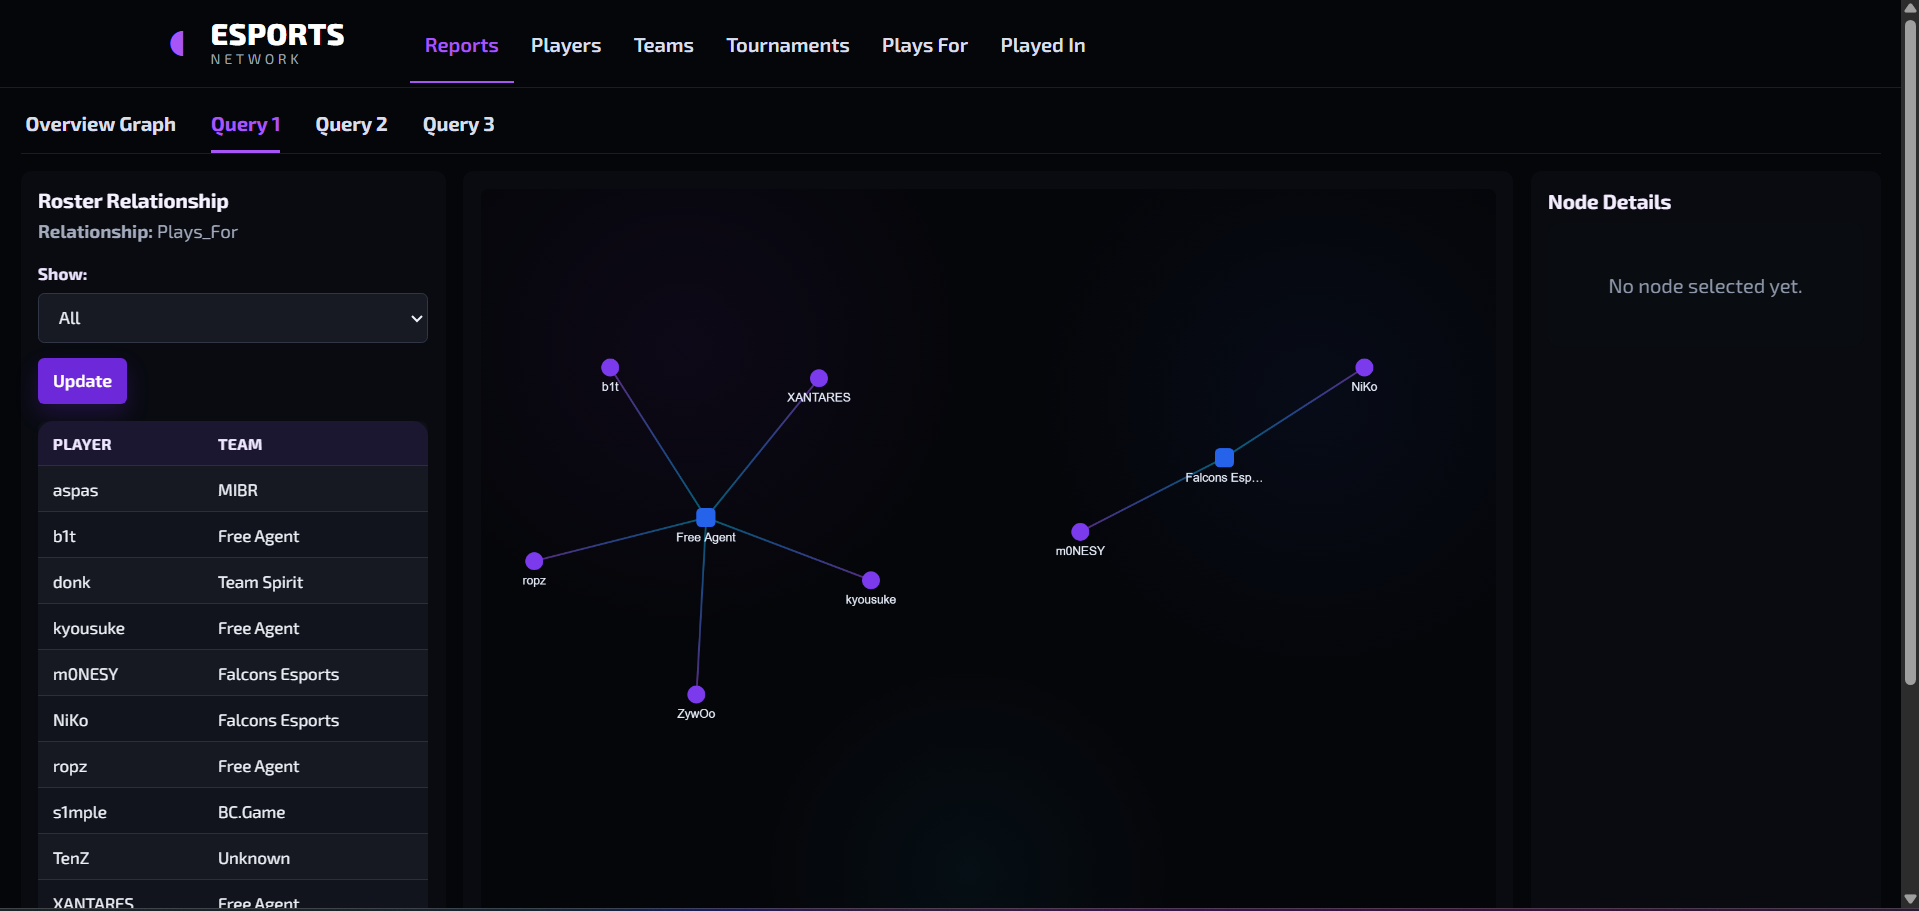
\includegraphics[width=1\linewidth]{images/ESports-Q1.png}
    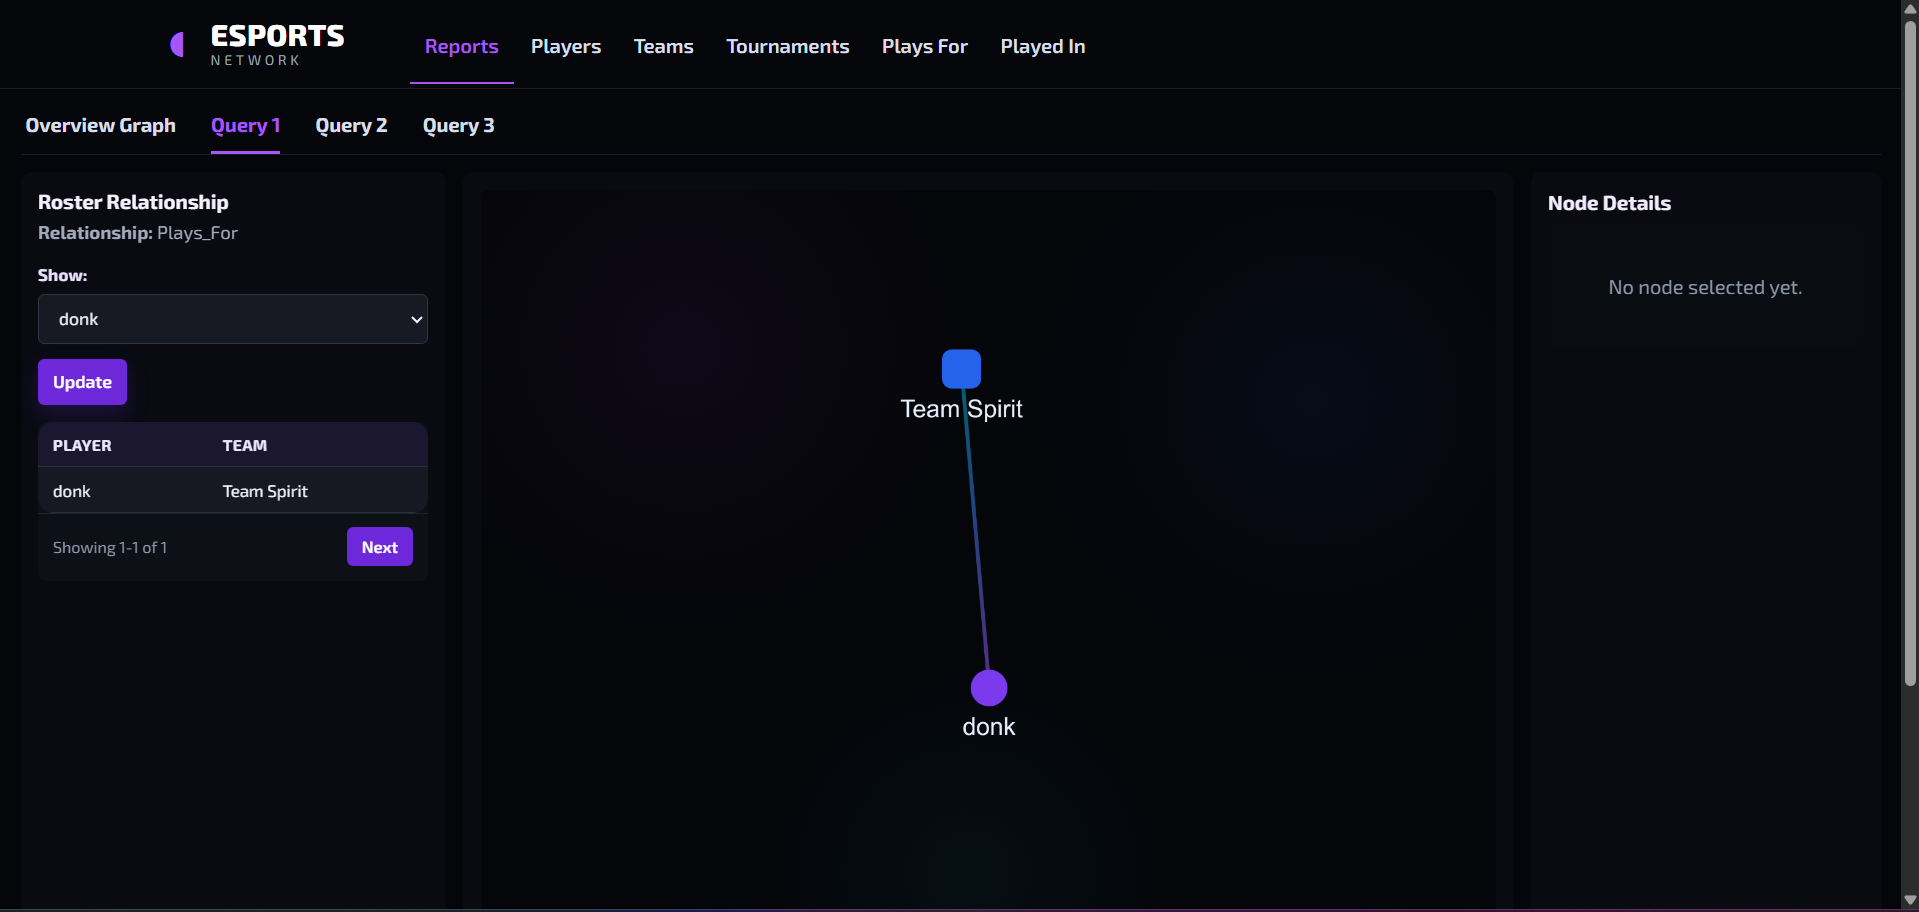
\includegraphics[width=1\linewidth]{images/ESports-Q1Example.png}
    \caption{Query 1 Webpage with Example}
    \label{fig:placeholder}
\end{figure}
\subsection{Query 2}
For the second analytical query we implemented a \textit{h-index filter}. Which takes a specific a specific number to represent the h-index. Then applies a filter on the teams and then presents that graphically with the tournaments and teams that participated in them. This is based on the analytical tool by the same named used in research paper influence measurement. The first two queries are executed to gather the number of \textit{Played In} edges each team has. If filtering by the number of wins the third query is executed to determine number of wins within the edges. If filtering by the participation the last query is executed to check the number of edges total. Figure 6 showcases the web pages them self, including both types of h-index filters.
\begin{verbatim}
SELECT SourceNodeID, COUNT(DISTINCT TargetNodeID) 
    AS participant_count
    FROM Edges
    WHERE EdgeType = "Played_In"
    GROUP BY SourceNodeID  
SELECT NodeID, Name, NodeType, Attributes
    FROM Nodes
    WHERE NodeType = "Team"
    ORDER BY Name

    
SELECT e.EdgeID, e.SourceNodeID, e.TargetNodeID,
    tr.Name AS tournament_name, 
    tr.Attributes AS tournament_attributes
    FROM Edges e
    JOIN Nodes tr ON tr.NodeID = e.SourceNodeID
    WHERE e.EdgeType = "Won_By"
      AND tr.NodeType = "Tournament"
    ORDER BY tr.Name
    
SELECT e.EdgeID, e.SourceNodeID, e.TargetNodeID,
    tr.Name AS tournament_name, 
    tr.Attributes AS tournament_attributes
    FROM Edges e
    JOIN Nodes tr ON tr.NodeID = e.SourceNodeID
    WHERE e.EdgeType = "Played_In"
      AND tr.NodeType = "Tournament"
    ORDER BY tr.Name
\end{verbatim}
\begin{figure}[H]
    \centering
    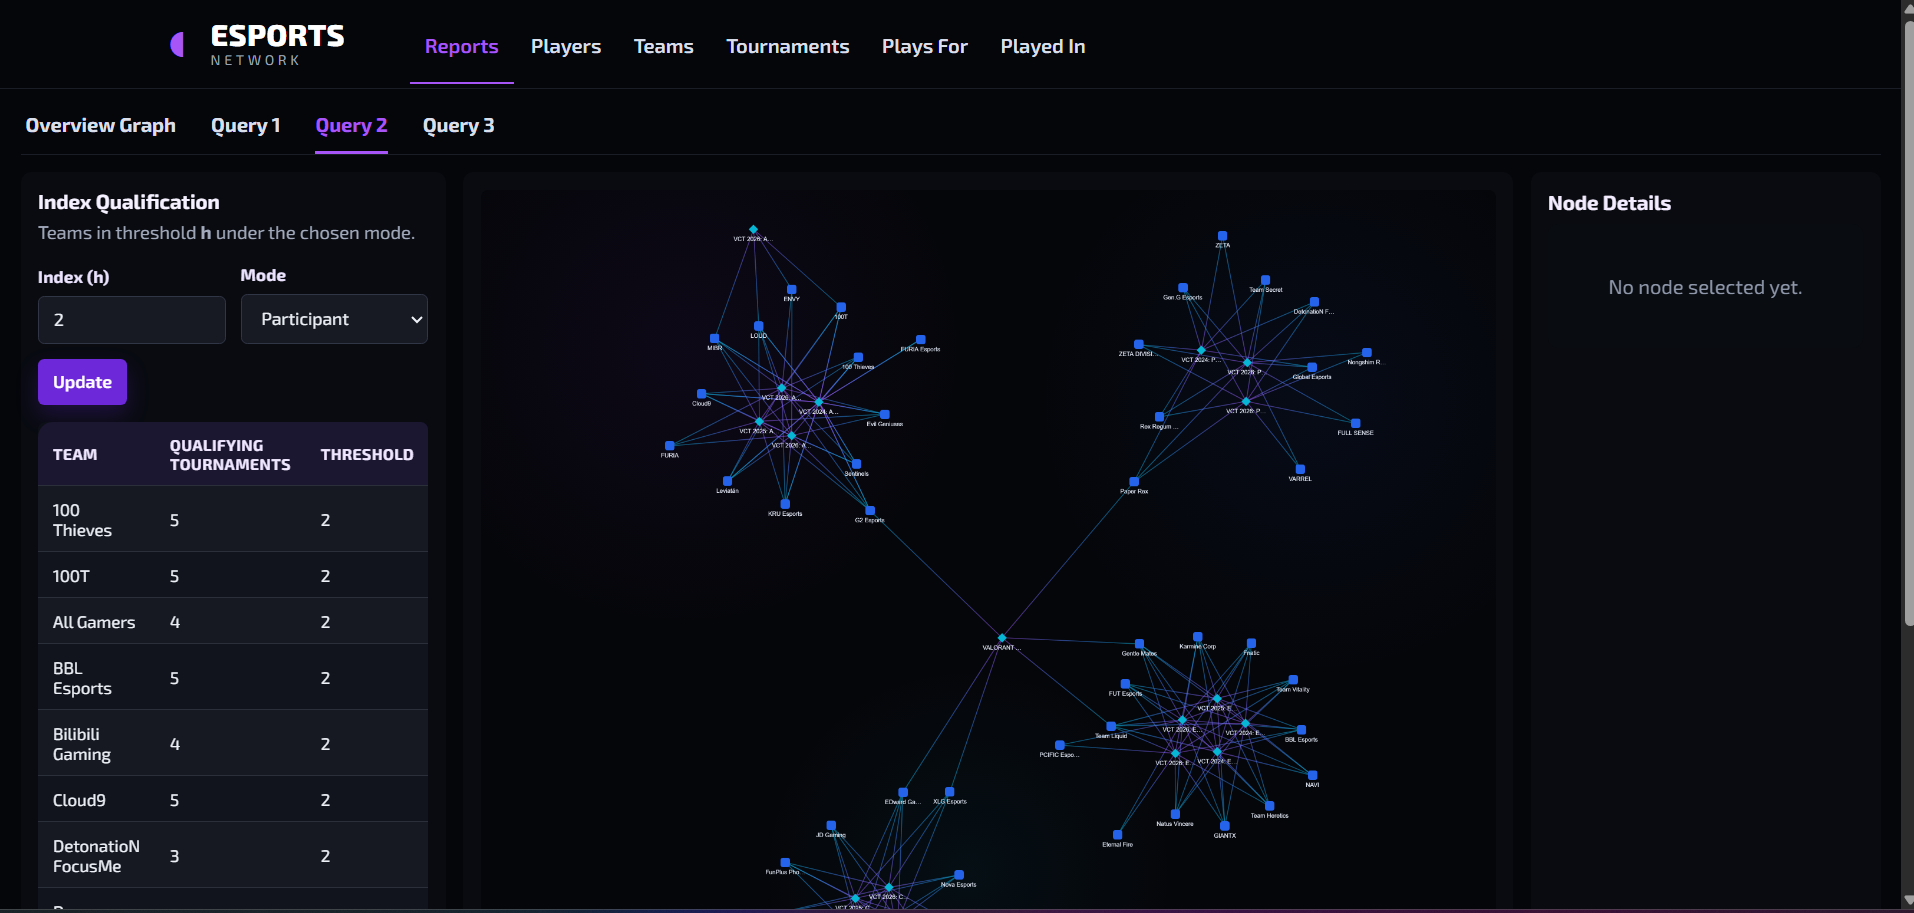
\includegraphics[width=1\linewidth]{images/ESports-Q2.png}
    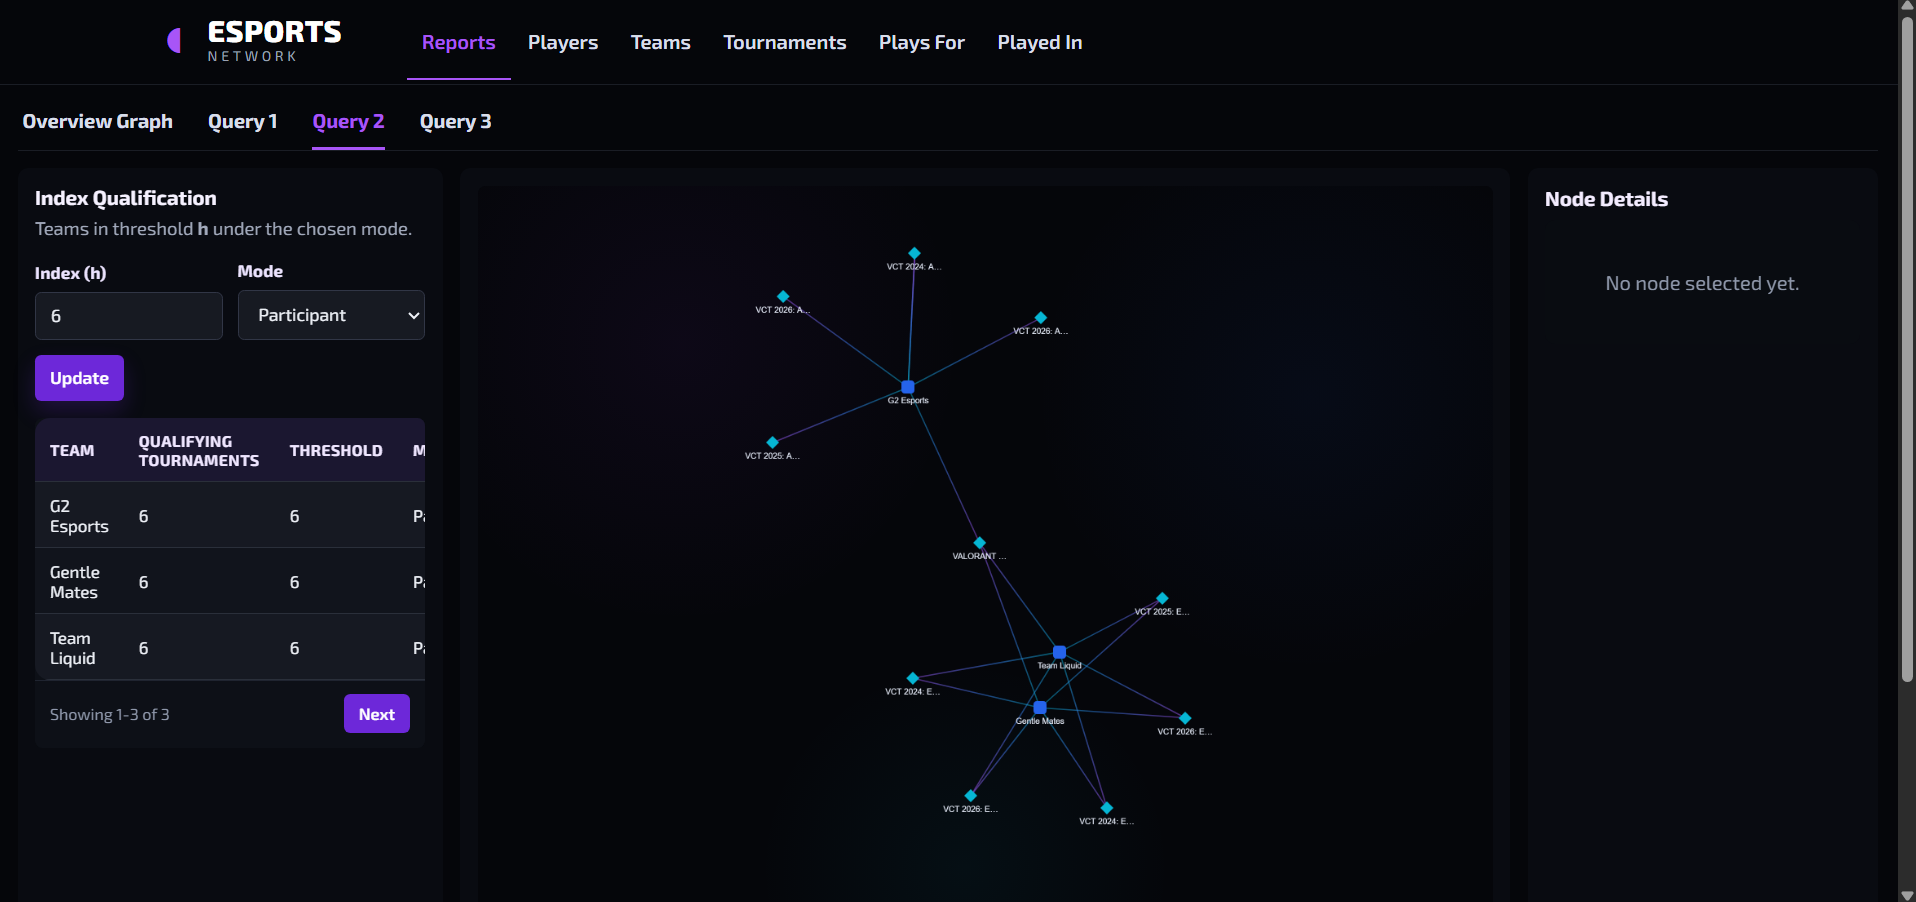
\includegraphics[width=1\linewidth]{images/ESports-Q2Example1.png}
    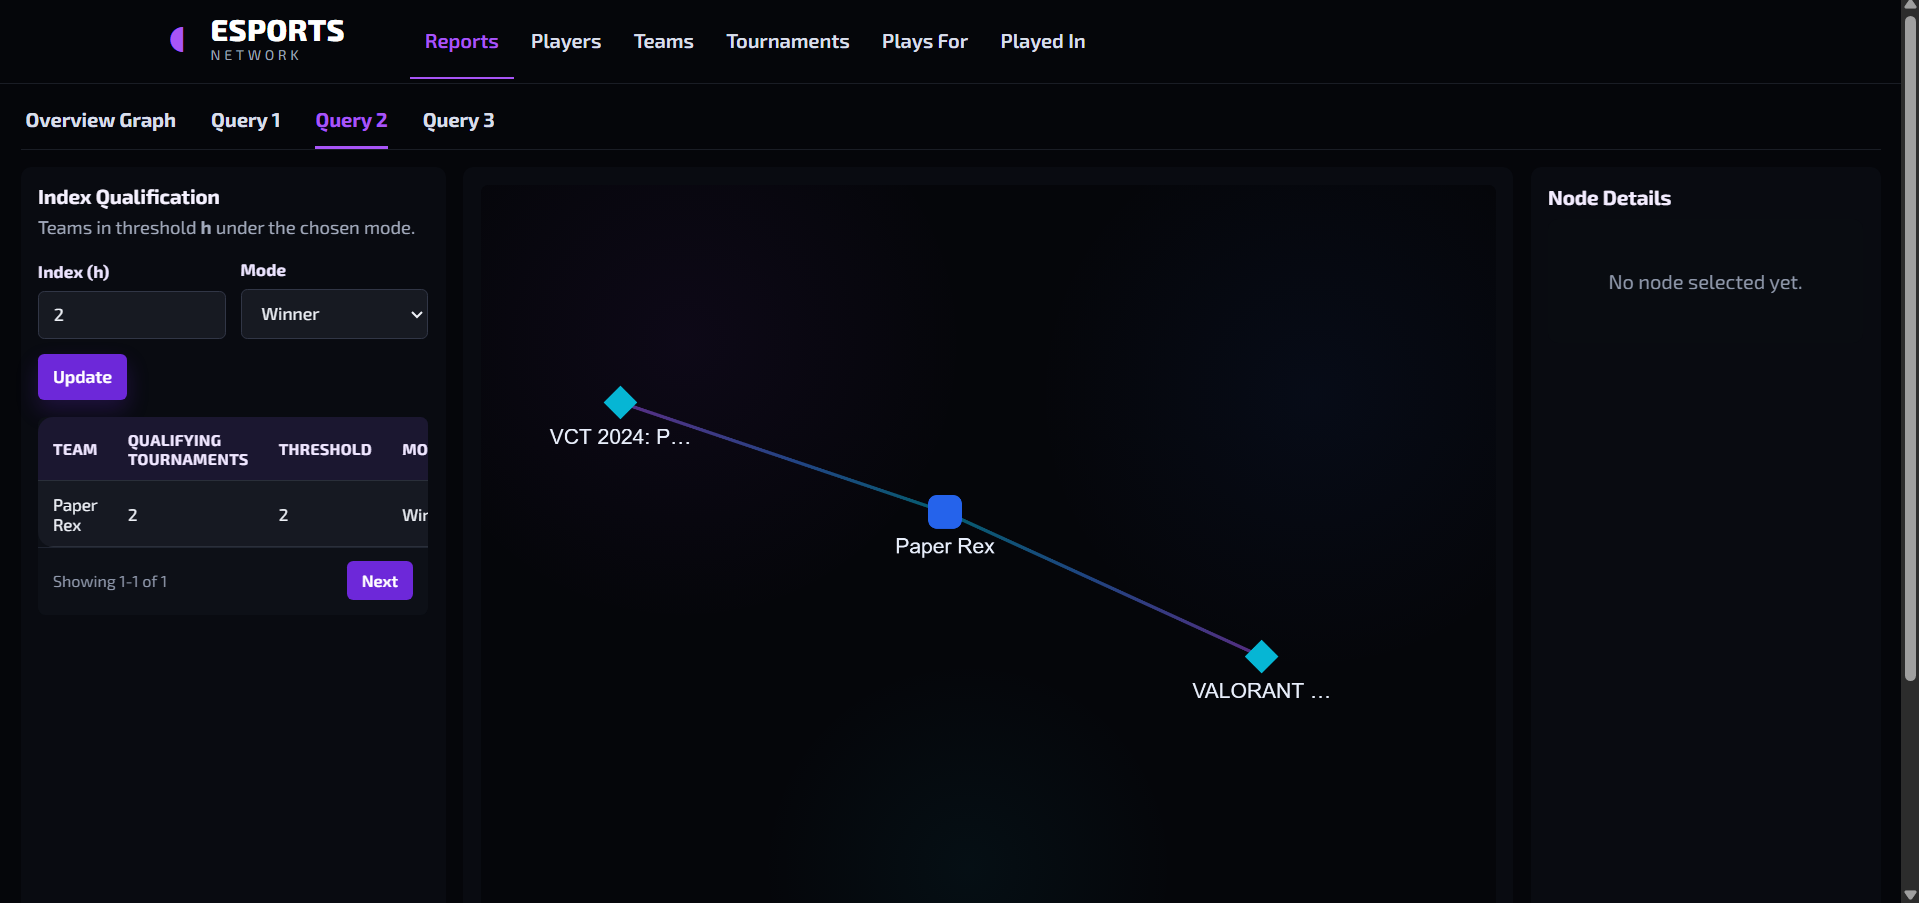
\includegraphics[width=1\linewidth]{images/ESports-Q2Example2.png}
    \caption{Query 2 Webpage with Examples}
    \label{fig:placeholder}
\end{figure}
\subsection{Query 3}
The last analytical query we implemented is a \textit{Q1 Tournament Influence Network}. Which is based on the \textit{Q1 Journel Influence Network} used by research paper databases. We defined a Q1 tournament as a tournament where the prize pool is greater than 1 million dollars. The influence network of a Q1 tournament is all teams that participated in that tournament. For this query the below statements are executed. The first query gets all the tournaments from the database. The second gets the team nodes and the last query gets the respective edges. The tournaments are then filtered by the prize pool size. Figure 7 depicts the respective web page.

\begin{verbatim}
SELECT DISTINCT n.NodeID, n.Name, n.NodeType, n.Attributes
    FROM Nodes n
    JOIN GraphMemberships gm ON gm.NodeID = n.NodeID
    WHERE gm.GraphID = 3
    AND n.NodeType = "Tournament"
    ORDER BY n.Name

SELECT DISTINCT n.NodeID, n.Name, n.NodeType, n.Attributes
    FROM Nodes n
    JOIN GraphMemberships gm ON gm.NodeID = n.NodeID
    WHERE gm.GraphID = 3
    AND n.NodeType = "Team"
    ORDER BY n.Name

SELECT DISTINCT e.EdgeID, e.SourceNodeID, e.TargetNodeID, 
    e.EdgeType
    FROM Edges e
    JOIN GraphMemberships gm ON gm.EdgeID = e.EdgeID
    WHERE gm.GraphID = 3
    AND e.EdgeType IN ("Played_In", "Won_By")
    ORDER BY e.EdgeID
\end{verbatim}

\begin{figure}[H]
    \centering
    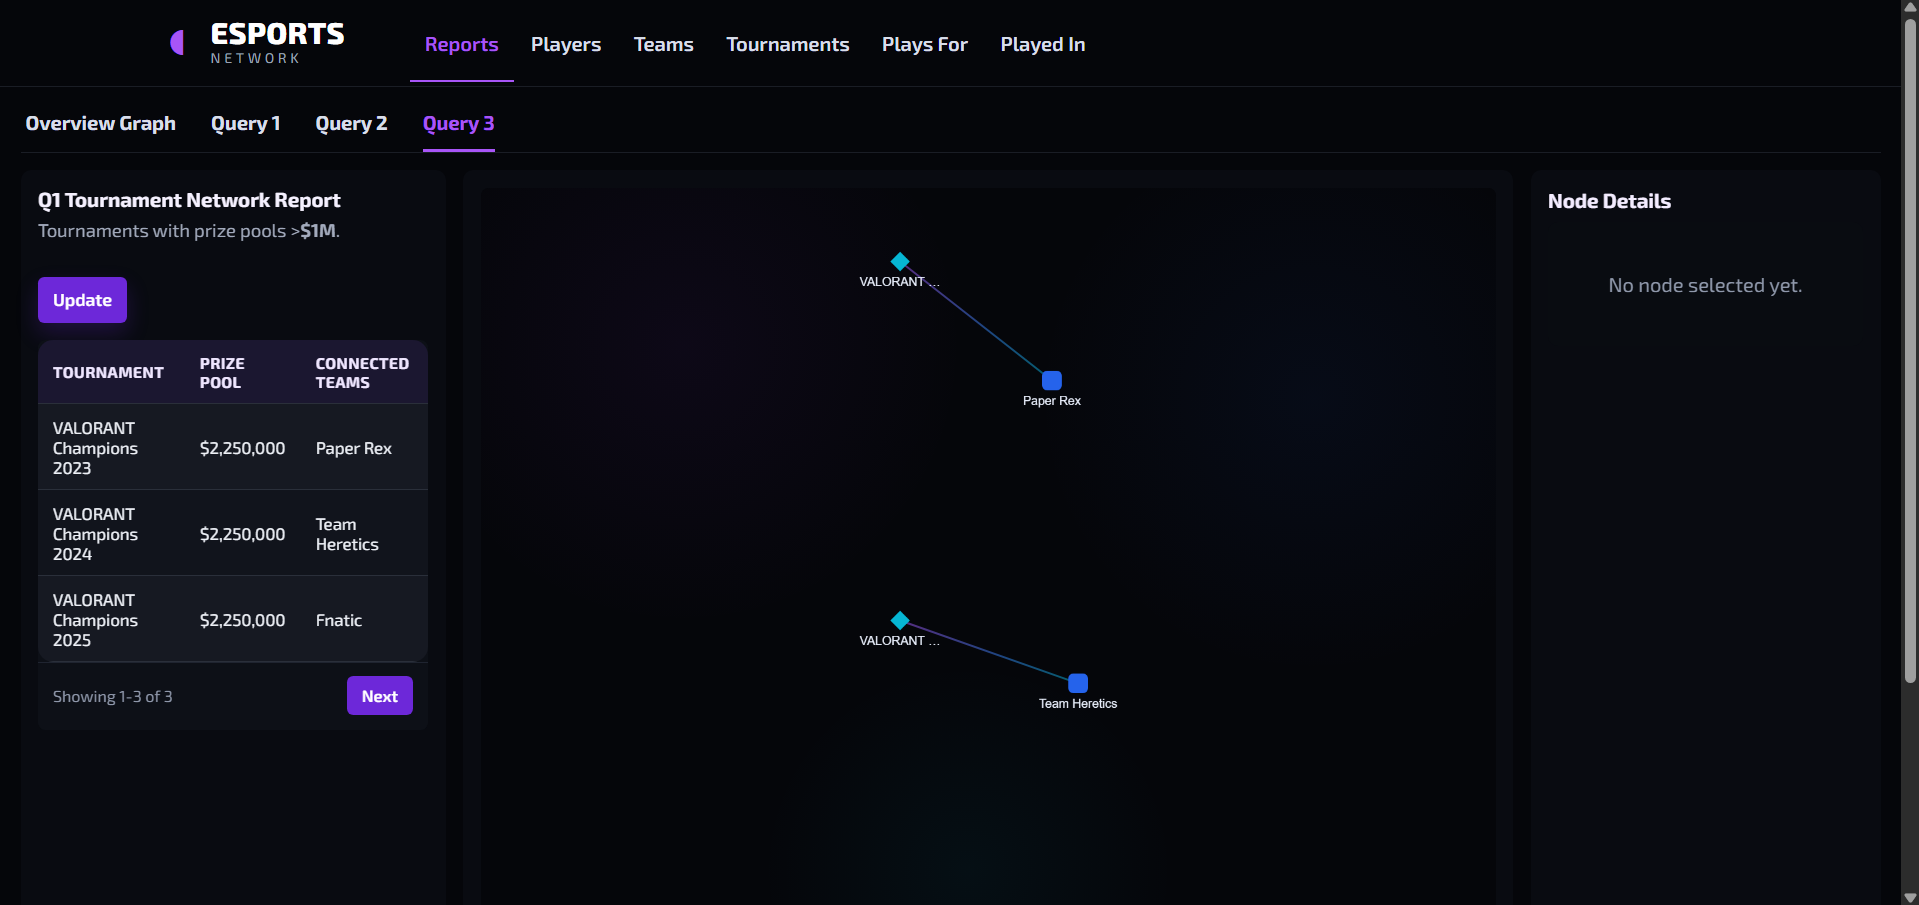
\includegraphics[width=1\linewidth]{images/ESports-Q3.png}
    \caption{Query 3 Webpage with Example}
    \label{fig:placeholder}
\end{figure}

\subsection{Timeline Comparison}
Below is the timeline outlined in phase one.
\begin{itemize}
    \item Phase 1: 
    \begin{itemize}
        \item Initial Design Presentation\\Date: March 3rd
        \item Initial Project Outline Report\\Date: March 7th
    \end{itemize}
    \item Phase 2: 
    \begin{itemize}
        \item Working Prototype Presentation\\Date: March 24th
        \item General Design Report\\Date: March 28th
    \end{itemize}
    \item Phase 3:
    \begin{itemize}
        \item Fully Function Prototype Presentation\\Date: April 21st
        \item Expanded Design Report\\Date: April 25th
    \end{itemize}
    \item Phase 4:
    \begin{itemize}
        \item Final Project Demo\\Date: May 7th
        \item Finalized Project Report\\Date: May 10th
    \end{itemize}
\end{itemize}
Since we have finished the project on time it's clear we more or less have matched this schedule. We started by outlining the project's central idea and the timeline itself which comprised phase one. Next we moved towards creating the initial prototype and database, allowing for the initial create, read, update, delete operations. This prototype also included initial Cytoscape integration on the webpage. This comprised phase 2. Once the initial prototype was completed we then overhauled the schema to what was discussed earlier in this report. This also included the first and second analytical query implementation. This phase included most of the learning curve as we familiarized with the unknown technology, Cytoscrape. Similarly the first phases of the web scrappers were completed at this phase. That concluded phase three. Finally we made a final sprint to finish the last analytical query as well as create the rest of the web scrappers. However, we then completely overhauled the web scrapper as it was inefficient with how it accessed the url and html data. Finally, we polished the overall look of the project as well as smaller UI features. Which concluded phase four with the final product.
\section{Conclusion}
E-Sports has rapidly evolved into a global form of entertainment across titles such as \textit{League of Legends}, \textit{Counter-Strike}, and \textit{Dota 2}. Despite this growth, the analytical infrastructure supporting e-sports still lags behind traditional sports. The E-Sports Competitive Network directly addresses this limitation by introducing a relational database designed to model the relationships between players, teams, and tournaments across multiple games. These relationships are showcased through an updated relationship schema and tech stack. The E-Sports Competitive Network allows for mass population of it's database through a set of custom developed web scrappers and manual insertion through its web pages. The E-Sports Competitive Network features three key queries, the teammate network which showcases how players are related across teams. A h-index filter to showcase teams based on the number or tournaments they've participated in as well as won. Lastly, the Q1 journal influence network which showcases all teams that have participated in a tournament with a prize pool over 1 million dollars. The E-Sports Competitive Network lays the groundwork for more advanced analytical tools that can benefit coaches, analysts, and researchers.
\bibliographystyle{ACM-Reference-Format}
\bibliography{references.bib}
\cite{Shannon2003Cytoscape}
\cite{playwright_python}

\end{document}
\endinput
%%
%% End of file `main.tex'.
